\chapter{Metodologia: Disseny Experimental}
\label{chap:metodologia}

Aquest capítol fixa l'entorn, la matriu, les mètriques i ---amb fórmula, no amb una cita d'una línia--- per què el gauntlet usa 10.000 partides per cel·la i 1.000 quan intervé MCTS. Sense aquest protocol, els nombres del Capítol~\ref{chap:resultats} no es poden llegir.

% ============================================================
\section{Entorn de Simulació}
\label{sec:entorn}

\subsection{Arquitectura client--servidor de Pokémon Showdown}

Showdown~\cite{pokemon_showdown} és una aplicació Node.js amb protocol WebSocket. En recerca s'executa localment:

\begin{verbatim}
  node pokemon-showdown start --port 8000 --no-security
\end{verbatim}

\texttt{--no-security} desactiva autenticació. Cada instància ocupa un port TCP i guarda l'estat de les batalles en RAM. Els missatges són text amb delimitador \texttt{|}:

\begin{verbatim}
  |move|p1a: Pikachu|Thunderbolt|p2a: Gyarados
  |-damage|p2a: Gyarados|23/100
  |-supereffective|p2a: Gyarados
  |turn|5
\end{verbatim}

El missatge crític per a l'agent és \texttt{|request|}, un JSON amb moviments legals, PP, stats \emph{pròpies} i HP. Les stats i l'objecte del rival \textbf{no} hi són: això és $\Omega\subset S$.

L'agent respon amb \texttt{/choose move 1}, \texttt{/choose switch 4} o \texttt{/choose move 1 terastallize}. El servidor resol el torn de forma atòmica (prioritat, velocitat, dany, secundaris) i emet el log.

\begin{figure}[H]
    \centering
    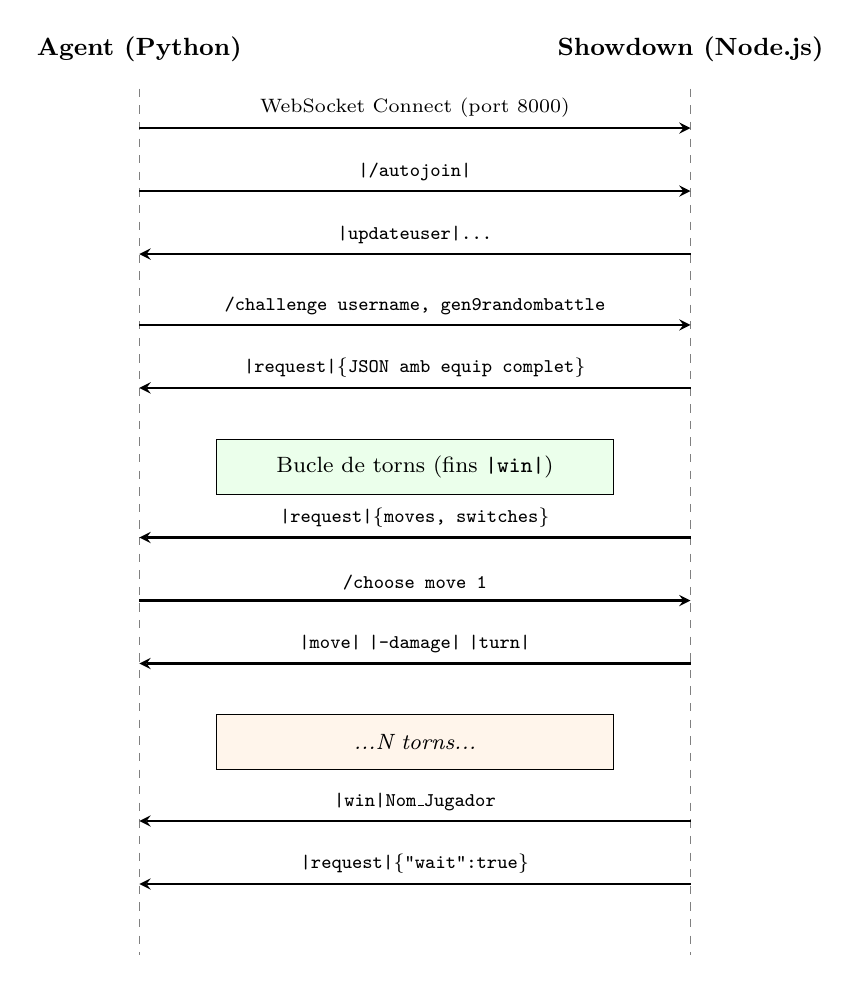
\begin{tikzpicture}[
        node distance=1.1cm, auto, font=\footnotesize,
        block/.style={rectangle, draw, fill=blue!5, text width=4.8cm, align=center, minimum height=0.7cm},
        msg/.style={->, thick, >=stealth},
        lbl/.style={font=\scriptsize, midway}
    ]
        \node[font=\small\bfseries] (agent_title) at (0,0) {Agent (Python)};
        \node[font=\small\bfseries] (server_title) at (7,0) {Showdown (Node.js)};
        \draw[dashed, gray] (0,-0.5) -- (0,-11.5);
        \draw[dashed, gray] (7,-0.5) -- (7,-11.5);

        \draw[msg] (0,-1) -- node[above, lbl]{WebSocket Connect (port 8000)} (7,-1);
        \draw[msg] (0,-1.8) -- node[above, lbl]{\texttt{|/autojoin|}} (7,-1.8);
        \draw[msg, <-] (0,-2.6) -- node[above, lbl]{\texttt{|updateuser|...}} (7,-2.6);

        \draw[msg] (0,-3.5) -- node[above, lbl]{\texttt{/challenge username, gen9randombattle}} (7,-3.5);
        \draw[msg, <-] (0,-4.3) -- node[above, lbl]{\texttt{|request|\{JSON amb equip complet\}}} (7,-4.3);

        \node[block, fill=green!8] at (3.5,-5.3) {Bucle de torns (fins \texttt{|win|})};

        \draw[msg, <-] (0,-6.2) -- node[above, lbl]{\texttt{|request|\{moves, switches\}}} (7,-6.2);
        \draw[msg] (0,-7.0) -- node[above, lbl]{\texttt{/choose move 1}} (7,-7.0);
        \draw[msg, <-] (0,-7.8) -- node[above, lbl]{\texttt{|move|} \texttt{|-damage|} \texttt{|turn|}} (7,-7.8);

        \node[block, fill=orange!8] at (3.5,-8.8) {\textit{...N torns...}};

        \draw[msg, <-] (0,-9.8) -- node[above, lbl]{\texttt{|win|Nom\_Jugador}} (7,-9.8);
        \draw[msg, <-] (0,-10.6) -- node[above, lbl]{\texttt{|request|\{"wait":true\}}} (7,-10.6);
    \end{tikzpicture}
    \caption{Protocol WebSocket d'una batalla local. L'estat viu a la RAM del procés Node.js; el servidor és determinista donats inputs i llavor RNG.}
    \label{fig:cicle_batalla}
\end{figure}

Latència típica d'un torn heurístic en local: $<5$~ms. MCTS, amb 100 \texttt{LocalSim}, és un altre ordre de magnitud (secció~\ref{sec:n_10k}).

\subsection{poke-env}

poke-env~\cite{poke_env} encapsula el protocol. El desenvolupador implementa \texttt{choose\_move(battle)}. Internament: parser $\rightarrow$ objecte \texttt{Battle} $\rightarrow$ ordre \texttt{/choose ...}.

\begin{figure}[H]
    \centering
    \begin{tikzpicture}[
        node distance=0.8cm, font=\footnotesize,
        box/.style={rectangle, draw, text width=3.2cm, align=center, minimum height=0.9cm},
        arr/.style={->, thick, >=stealth}
    ]
        \node[box, fill=red!8] (ws) {WebSocket cru};
        \node[box, fill=yellow!10, right=of ws] (parser) {\texttt{parse\_message}};
        \node[box, fill=blue!8, right=of parser] (battle) {\texttt{Battle}};
        \node[box, fill=green!8, below=of battle] (agent) {\texttt{choose\_move(battle)}};
        \node[box, fill=purple!8, left=of agent] (order) {\texttt{BattleOrder}};
        \node[box, fill=red!8, left=of order] (ws2) {\texttt{/choose ...}};
        \draw[arr] (ws) -- (parser);
        \draw[arr] (parser) -- (battle);
        \draw[arr] (battle) -- (agent);
        \draw[arr] (agent) -- (order);
        \draw[arr] (order) -- (ws2);
    \end{tikzpicture}
    \caption{Pipeline intern de poke-env.}
    \label{fig:pokeenv_arch}
\end{figure}

Concurrència: \texttt{asyncio} i \texttt{max\_concurrent\_battles}. Pin \textbf{0.11.x}. El fork de Pokechamp s'injecta només quan cal \texttt{LocalSim} (MCTS); el motor de mecàniques continua sent el Node.js de Showdown. \texttt{strict\_battle\_tracking=False} evita que un desajust de protocol mati un worker de 10k.

\subsection{Què observa l'agent}

\begin{table}[H]
    \centering
    \small
    \begin{tabular}{|l|p{10cm}|}
    \hline
    \textbf{Visible} & \textbf{Detall} \\ \hline
    Equip propi & HP, stats, item, ability, boosts, PP, status. \\ \hline
    Rival actiu & Espècie, HP\%, tipus, moviments \emph{ja usats}, status visible. \\ \hline
    Preview & Les sis espècies rivals (no el set). \\ \hline
    Camp & Clima, terrain, hazards, pantalles, Trick Room. \\ \hline
    \textbf{Ocult} & EVs/IVs/Nature rivals, item i ability fins que es revelen, moviments no usats, ordre exacte del banc. \\ \hline
    \end{tabular}
    \caption{Observació per torn. El pool de sets de Random Battle redueix l'ocult a una mescla discreta, no a OU lliure.}
    \label{tab:variables_estat}
\end{table}

\subsection{Per què cal paral·lelisme}

Un sol procés Node.js satura cap a 20--30 batalles simultànies i acumula memòria (V8 no allibera del tot l'\textit{old generation}). El patró és \textbf{master--worker}: $N$ servidors, $N$ subprocessos Python, ports exclusius, CSV a disc cada chunk. Detall al Capítol~\ref{chap:implementacio}.

\begin{figure}[H]
    \centering
    \begin{tikzpicture}[
        node distance=1.5cm, font=\small,
        master/.style={rectangle, draw, fill=blue!10, text width=3.5cm, align=center, minimum height=1cm},
        worker/.style={rectangle, draw, fill=green!10, text width=2.5cm, align=center, minimum height=0.8cm},
        server/.style={rectangle, draw, fill=orange!10, text width=2.5cm, align=center, minimum height=0.8cm},
        disk/.style={cylinder, draw, fill=gray!10, shape border rotate=90, aspect=0.3, minimum height=0.8cm, minimum width=1.5cm, align=center}
    ]
        \node[master] (master) {Master\\(\texttt{benchmark.py})};
        \node[worker, below left=1.5cm and 0.5cm of master] (w1) {Worker 1};
        \node[worker, below=1.5cm of master] (w2) {Worker 2};
        \node[worker, below right=1.5cm and 0.5cm of master] (wn) {Worker N};
        \node[server, below=0.8cm of w1] (s1) {Showdown 8000};
        \node[server, below=0.8cm of w2] (s2) {Showdown 8001};
        \node[server, below=0.8cm of wn] (sn) {Showdown 800N};
        \node[disk, right=2cm of master] (csv) {CSV};
        \draw[->, thick] (master) -- (w1);
        \draw[->, thick] (master) -- (w2);
        \draw[->, thick] (master) -- (wn);
        \draw[<->, thick] (w1) -- (s1);
        \draw[<->, thick] (w2) -- (s2);
        \draw[<->, thick] (wn) -- (sn);
        \draw[->, dashed] (w1.east) -- ++(0.3,0) |- (csv);
        \draw[->, dashed] (w2.east) -- ++(0.15,0) |- (csv);
        \draw[->, dashed] (wn.north east) -- ++(0.5,0.3) -| (csv);
    \end{tikzpicture}
    \caption{Master--worker: aïllament de procés, un Showdown per worker, persistència incremental.}
    \label{fig:infraestructura}
\end{figure}

% ============================================================
\section{Per què 10.000 partides (i per què 1.000 per a MCTS)}
\label{sec:n_10k}

Aquesta secció és el cor metodològic. No n'hi ha prou amb «hem fet moltes partides». Cal dir què es pot afirmar i què és soroll.

\subsection{Cada batalla és un Bernoulli}

El resultat que entra al WR és binari: $W_i\in\{0,1\}$, victòria de l'agent fila. Sigui $p=\mathbb{E}[W]$. L'estimador $\hat p = n^{-1}\sum W_i$ té
\begin{equation}
    \mathrm{Var}(\hat p)=\frac{p(1-p)}{n}\le \frac{1}{4n}.
\end{equation}
L'interval de Wald al 95\% és
\begin{equation}
    \hat p \;\pm\; 1{,}96\sqrt{\frac{\hat p(1-\hat p)}{n}}.
\end{equation}
El cas pitjor (màxima variància) és $p=0{,}5$:
\begin{equation}
    1{,}96\sqrt{\frac{0{,}25}{n}}.
    \label{eq:ci95}
\end{equation}
Substitució directa:

\begin{itemize}
    \item $n=10.000$: $1{,}96\sqrt{0{,}25/10.000}=1{,}96\times 0{,}005=0{,}0098$ $\rightarrow$ \textbf{$\pm 0{,}98$ punts percentuals}.
    \item $n=1.000$: $1{,}96\sqrt{0{,}25/1.000}\approx 0{,}0310$ $\rightarrow$ \textbf{$\pm 3{,}10$~pp}.
    \item $n=100$: $\approx\pm 10$~pp.
\end{itemize}

\begin{table}[H]
\centering
\caption{Amplada de l'interval de confiança del 95\% per a una proporció binomial en el cas pitjor ($p=0{,}5$). Fórmula: $\pm 1{,}96\sqrt{0{,}25/n}$. El llindar de detecció és l'ordre de magnitud de la diferència que es pot distingir de manera fiable entre dos agents independents.}
\label{tab:ci_n}
\small
\begin{tabular}{rrll}
\toprule
\textbf{$n$ (partides)} & \textbf{IC 95\%} & \textbf{Detecta buits $\gtrsim$} & \textbf{Ús en aquest TFM} \\
\midrule
100     & $\pm 10$~pp  & $20$~pp & Prova de fum (desenvolupament); \textbf{mai} un resultat. \\
1.000   & $\pm 3{,}10$~pp & $6$~pp & Nivell de validació. Totes les cel·les amb \texttt{v18}/\texttt{v19}/\texttt{v20}. \\
5.000   & $\pm 1{,}39$~pp & $2{,}8$~pp & (no usat) \\
10.000  & $\pm 0{,}98$~pp & $2$~pp & Nivell de publicació. Cel·la per defecte del gauntlet. \\
20.000  & $\pm 0{,}69$~pp & $1{,}4$~pp & (no usat; cost doble per un guany marginal) \\
\bottomrule
\end{tabular}
\end{table}


Un buit observat de 2~pp entre dos agents independents a 10k és de l'ordre de dos errors estàndard: detectable. El mateix buit a 1k està \emph{dins} de l'IC. Un buit de 1~pp a 10k (p.~ex.\ \texttt{v1} vs \texttt{v2}) és compatible amb igualtat; que siguin equivalents és un resultat, no un fracàs del protocol.

Per a una taxa global sobre 253.000 partides, Wilson / Wald dona $\approx\pm 0{,}19$~pp. Això fa visibles salts de 0,5~pp (com \texttt{v16} vs \texttt{v15}) que \emph{no} importen tàcticament. El text distingeix «detectable a 253k» de «rellevant».

\subsection{El Pokédex no entra a la variància}

La intuïció «Gen~9 té 1.025 Pokémon, calen més partides que a Gen~1» és falsa per a un WR. $\mathrm{Var}(\hat p)$ depèn de $p$ i $n$, no de $|Pokedex|$, no del nombre de sets, no de si hi ha Tera. L'espai d'equips $C(n,6)$ és
\begin{center}
Gen~1: $\sim 1{,}5\times 10^{10}$\; · \;
Gen~9: $\sim 1{,}6\times 10^{15}$.
\end{center}
Ni 10.000 ni 253.000 «cobreixen» l'espai. No ho pretén. El que es cobreix és l'esperança de $W$ sota la llei amb què Showdown mostreja equips i RNG. La llei dels grans nombres i el TCL garanteixen la convergència de $\hat p$, no un cens de combinacions.

Les fonts de variància per partida ---equip, crit, miss, speed tie, roll--- queden absorbides pel Bernoulli. No cal modelar-les una a una per declarar un IC sobre el WR.

El mateix $n$ a totes les generacions seria una elecció de \emph{comparabilitat}, no de cobertura. Aquest TFM publica Gen~9.

\subsection{Tres nivells, i només dos entren als Resultats}

Durant el desenvolupament s'ha usat una escala de tres pisos. \textbf{Només el segon i el tercer apareixen com a nombres de tesi}, i el segon amb l'etiqueta explícita de validació.

\paragraph{Prova de fum ($n=100$).}
Comprova que el codi no peti, que Tera dispara, que el WR no és 5\% per un bug. IC $\pm 10$~pp. Una anècdota de «\texttt{v13} va fer 9/10 contra \texttt{v12}» \textbf{no és un resultat}. El gauntlet la desmenteix (48,85\%). El text la cita només com a advertiment.

\paragraph{Validació ($n=1.000$).}
IC $\pm 3{,}1$~pp; detecta buits $\gtrsim 6$~pp. És el pis de l'MCTS. No és el pis de publicació per a una disputa de 2~pp.

\paragraph{Tesi ($n=10.000$).}
IC $\pm 0{,}98$~pp; detecta $\gtrsim 2$~pp. Cel·la per defecte.

\subsection{El gauntlet real: 784 CSV}

Directori canònic: \texttt{data/benchmarks/all\_10k/gen9randombattle}.

\begin{itemize}
    \item 28 agents (Taula~\ref{tab:taxonomy} al capítol de resultats): 6 baselines, \texttt{v1}--\texttt{v14}, \texttt{v15}--\texttt{v17}, \texttt{v18}--\texttt{v20}, \texttt{v21}, \texttt{v22}.
    \item Matriu dirigida $28\times 28=784$ fitxers \texttt{\{agent\}\_vs\_\{opponent\}.csv}. Fila $=$ \emph{nosaltres} (\texttt{heuristic} al CSV).
    \item \textbf{Cel·la per defecte: 10.000 partides.}
    \item \textbf{Excepció: si qualsevol dels dos bàndols és \texttt{v18}, \texttt{v19} o \texttt{v20}, $n=1.000$.} Motiu: IS-MCTS fa 100 rollouts de 5 torns per decisió de cerca. El cost per partida és d'un a dos ordres per sobre d'una heurística. 1.000 és el pis de validació, no una «10k a mitges».
    \item Pool per a heurística / minimax / IL com a nosaltres: $25\times 10.000 + 3\times 1.000=\mathbf{253.000}$ partides. IC global $\approx\pm 0{,}19$~pp; IC d'una cel·la 10k $\pm 0{,}98$~pp.
    \item Pool MCTS com a nosaltres: $28\times 1.000=\mathbf{28.000}$. IC global $\approx\pm 0{,}58$~pp; IC de cel·la $\pm 3{,}1$~pp. Un buit $<3$~pp en una cel·la MCTS és soroll.
\end{itemize}

\textbf{Prohibició metodològica.} No es mesclen un WR global de 28k (MCTS) i un de 253k (resta) com si fossin la mateixa estimació. Per ordenar \texttt{v20} contra \texttt{v17} es llegeix la \emph{cel·la} (\texttt{v17} vs \texttt{v20} $=50{,}4\%$ a 1k; \texttt{v20} vs \texttt{v17} $=55{,}8\%$ a 1k; IC $\pm 3{,}1$). El rànquing global és una brúixola, no un veredicte de 0,8~pp.

\subsection{Recíprocs i autojoc}

Pokémon no és simètric en seient (preview, RNG, qui és \texttt{p1}). Per això existeixen \texttt{A\_vs\_B.csv} i \texttt{B\_vs\_A.csv} independents. La suma de WR ha de ser $\sim 100\%$ (típicament 99,3--100,9). L'autojoc ha de ser $\sim 50\%$ (49,3--50,5 a les heurístiques). Si fallés, el seient o el CSV estarien trencats. Al gauntlet, no fallen.

\subsection{El WR global no és un Elo humà}

La mitjana sobre 28 oponents \textbf{inclou \texttt{random} i \texttt{max\_power}}. Tothom hi té un 90--98\%. El 69\% de \texttt{v12} no és «nivell humà 69\%». Les comparacions que discriminen són: vs Abyssal, vs Simple Heuristic, vs \texttt{v12}/\texttt{v13}/\texttt{v14}, vs \texttt{v21}. L'Elo Bradley--Terry (secció~\ref{sec:metriques}) repondera per qualitat d'oponent; encara així, \texttt{random} hi és l'àncora 1000, no un jugador de ladder.

\subsection{Ladder humana}

Protocol separat, no una fila de la matriu. \texttt{v14} a la ladder pública, 431 partides, Capítol~\ref{chap:resultats}. $n=431$ té IC $\pm 4{,}6$~pp: serveix per dir «no som al 50\% contra humans», no per invertir \texttt{v12} vs \texttt{v14}.

% ============================================================
\section{Espais formals en Singles}
\label{sec:espais}

$|A|\le 9$ per torn, dinàmic. No hi ha producte cartesià de Dobles. L'observació és el JSON de \texttt{request} més l'historial de moviments revelats. El vector de 238 dimensions del wrapper PPO existeix al framework i \textbf{no} s'usa al gauntlet d'aquesta memòria: els agents mesurats decideixen sobre l'objecte \texttt{Battle} o sobre 1.150 features tabulars (IL).

% ============================================================
\section{Mètriques}
\label{sec:metriques}

\subsection{Primària: taxa de victòries}

$\widehat{\mathrm{WR}}=\hat p$. Interpretació qualitativa \emph{només} després de l'IC:

\begin{itemize}
    \item $\sim 50\%$ a 10k: no hi ha avantatge detectable.
    \item $55$--$60\%$ vs un baseline fort (Abyssal): avantatge real.
    \item $98\%$ vs \texttt{random}: no informa de res entre experts.
    \item $100\%$: impossible sota rolls de dany.
\end{itemize}

\subsection{Secundàries (telemetria)}

El CSV de batalla porta identitat, HP final, canvis voluntaris vs forçats, crits/miss/SE, i comptadors de paradigma:

\begin{itemize}
    \item Heurístiques: \texttt{hazard\_sets}, \texttt{setup\_uses}, \texttt{ko\_checks}, \texttt{matchup\_switches}, \texttt{terastallized}. \textbf{Forat d'esquema:} \texttt{setup}/\texttt{hazards} queden a 0 per a \texttt{v7}/\texttt{v8}/\texttt{v10}; no s'interpreta com a «mai posen roques».
    \item Cerca: \texttt{search\_moves}, \texttt{search\_switches}, \texttt{search\_diff} (l'acció jugada $\neq$ la sonda \texttt{v14}). La taxa d'\emph{override} és $\texttt{search\_diff}/(\texttt{search\_moves}+\texttt{search\_switches})$ entre els torns que la cerca ha disparat.
    \item IL: \texttt{xgb\_stays}, \texttt{xgb\_switches}, \texttt{ko\_guards}, \texttt{loop\_guards}.
\end{itemize}

Aquestes columnes són el que permet dir «la cerca només corre el 16\% dels torns» en lloc de «és un agent de cerca».

\subsection{Elo Bradley--Terry}

No és l'Elo de ladder de Showdown. És un model de força sobre la matriu dirigida, àncora \texttt{random}${}=1000$, ambdós seients~\cite{elo_rating}. MCTS hi té menys partides (56k vs 506k). És un resum, no una substitució de les cel·les.

% ============================================================
\section{Disseny dels experiments}
\label{sec:disseny_experiments}

La taxonomia completa dels 28 agents (IDs, paradigma, una frase) és la Taula~\ref{tab:taxonomy} al capítol de resultats. Format únic: \texttt{gen9randombattle}. Sense Dobles. Sense PPO a la matriu.

Cada parella $(A,B)$ genera dos fitxers. Equips aleatoris del servidor. Ordre de seient fixat pel nom del fitxer, no barrejant $A$ i $B$ al mateix CSV.

Baselines: \texttt{random} (sòl), \texttt{max\_power} (golós), \texttt{one\_step}/\texttt{safe\_one\_step} (dany d'un pas; el «safe» evita el penjament de LocalSim de Pokechamp), \texttt{abyssal} i \texttt{simple\_heuristic} (el rival publicat de regles; en aquest gauntlet queden empatats amb \texttt{v14} a l'Elo).

No s'inclouen agents LLM al round-robin: la latència d'Ollama trenca el pressupost de 10k.

PPO: fora. La comparació futura prevista és contra \texttt{v12}, el sostre bot-contra-bot, no contra els 28.

% ============================================================
\section{Fases de desenvolupament (el que s'ha mesurat)}
\label{sec:fases}

\begin{enumerate}
    \item Heurístiques \texttt{v1}--\texttt{v14} com a ablació.
    \item Minimax 1-ply \texttt{v15}--\texttt{v17} sobre \texttt{v14}.
    \item IS-MCTS \texttt{v18}--\texttt{v20}, mateix professor, $n=1.000$.
    \item IL \texttt{v21}--\texttt{v22}, mateix macro, dues execucions.
    \item Ladder \texttt{v14} vs humans (pilot).
\end{enumerate}

El capítol d'implementació tradueix cada fase a codi. El de resultats no torna a explicar el protocol sencer, però \textbf{recorda $n=1.000$ cada cop que apareix MCTS}.
